\documentclass[a4paper]{article}
\usepackage[english]{babel}
\usepackage[utf8]{inputenc}
\usepackage{amsmath}
\usepackage{graphicx}
\usepackage{tikz}
\usepackage{dot2texi}
\usepackage{pgfplots}
\usepackage{algorithm}
 \usepackage{verbatim}
\usepackage{graphicx}
\usepackage{color}
\usepackage{epsfig}
\usepackage{multirow}
\usepackage{amsfonts}
\usepackage{hyperref}
\usepackage{wrapfig}
\usepackage{algpseudocode}
\usepackage[colorinlistoftodos]{todonotes}
\usepackage{geometry}
 \geometry{
 a4paper,
 total={210mm,297mm},
 left=20mm,
 right=20mm,
 top=10mm,
 bottom=15mm,
 }



\title{Modeling Blockchain based Lottery protocol in Tamarin}
\author{Parag Bansal}
\date{June 2017}
\begin{document}
\maketitle
\section{Bitcoin}

Bitcoin is digital currency protocol introduced in 2008. It is a decentralised protocol which lacks any central authority and the list of all the transactions are kept in publicly available ledger called blockchain. Transfer of money from one party to another party is done by requesting a transaction, digitally signed by the private key. Miners verify such request and club many such request to form a block, and blocks are then linked into the blockchain.\\

\subsection{Currency Flow}

\begin{wrapfigure}{r}{0.5\textwidth}
  \begin{center}
    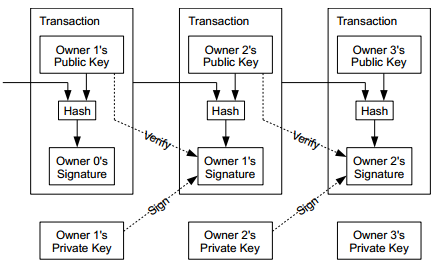
\includegraphics[width=0.48\textwidth]{bitcoin.png}
  \end{center}
  \caption{Transaction structure}
\end{wrapfigure}
A coin owner transfers coins by digitally signing a hash digest of the previous transaction(unspent) and the public key of next owner. New coins are generated due to mining process, miner receives a block reward on solving a block puzzle.\\ Note that syntax of bitcoin allows for more advanced transactions than simply transferring money. Each bitcoin transaction has an output script(A boolean function) associated with it, which must be evaluated to true for redeeming that transaction. In simple case, the boolean function requires signature to be evaluated to true, but you can specify advanced conditions. Every transactions take few(more than or equal to one) previously posted transactions which are not redeemed as input, along with the input(signature simply) to satisfy the boolean function of each input transaction.
\subsection{Double Spending}
The most important problem with any digital currency is the problem of double spending since coins are just bit string, owner can spend it multiple times. This can be avoided if everyone has access to a trusted ledger which keeps track of transactions but that would defeat the purpose, as we are looking for decentralized protocol. Bitcoin tackles this problem by using blockchain. Miners pick unconfirmed transactions and put them in a block after solving a moderately difficult block puzzle. Note that, at time of creating a block miner verify, whether the input transactions have not been redeemed previously and all the boolean functions of this transaction evaluates to true.\\
Since many miners are simultaneously working on solving block, it might be the case that multiple miners end up solving a block simultaneously. In such cases blockchain forks to form a tree like structure. Longest length path in this tree is always the accepted blockchain, and miners try to append the block to longest path.\\
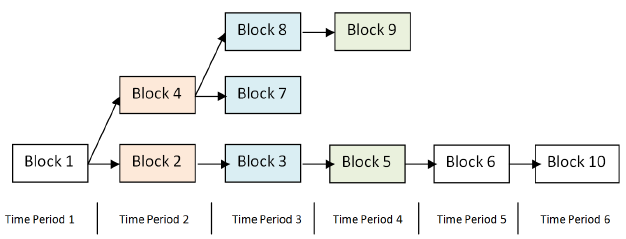
\includegraphics[width =0.5\textwidth]{bitcoin2.png}
\\If an adversary has to do a double spending attacks then it has to invalidate all the blocks that come after the block which contains the transaction, i.e. miner has to create a longer blockchain and mine a lot of blocks. Note that, a miner is in race with rest of the network so to mine a large number of blocks faster than other, it should have access to more 51\% of world's computing power. 
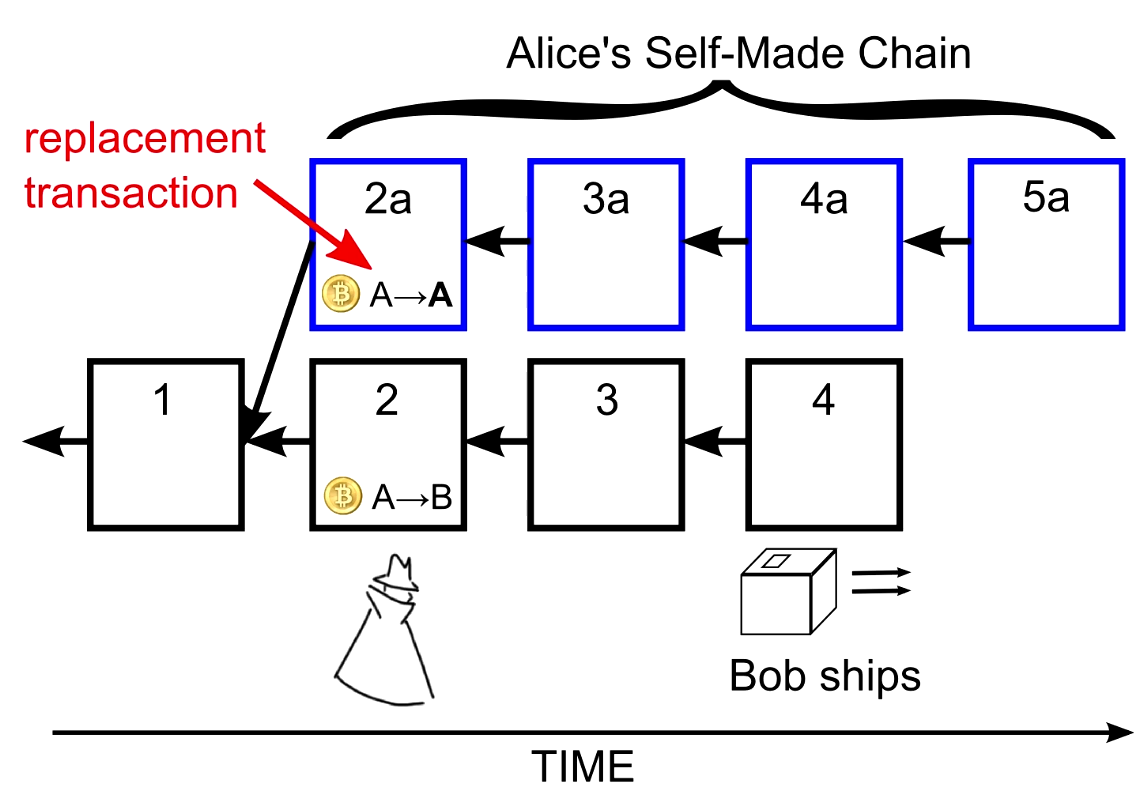
\includegraphics[width = 0.5\textwidth]{bitcoin3.png}
\section{Lottery Protocol}
\section{Tamarin Model}

\end{document}